\chapter{Background}
\label{cap:background}

In this chapter, we briefly describe the main fundamental concepts and technologies related to this work. Specifically, we describe the attack scenarios we considered during the design and evaluation, the Zeek network security monitoring system, and the P4 language for Programmable Data Planes.

\section{Cyberattacks}

Cyberattacks are constantly increasing, especially in a connected world, where work-from-home becomes more common every day. In this scenario, it is paramount to devise effective and efficient detection and mitigation mechanisms for all sorts of attacks, the focus of this work. Considering the use cases explored throughout this manuscript. Next, we briefly revisit the ``anatomy'' of specific attacks of interest.

\subsubsection*{FTP Bruteforce Attack}
\label{sec:bg:ftp_bruteforce}

FTP Bruteforce attacks are a common method of gaining unauthorized access to FTP servers. This attack consists of multiple and coordinated attempts to log on to a server, each time trying a new potential password. An attacker tries all or various combinations of passwords until one of them is accepted, effectively discovering someone's password \cite{FtpBruteforceAttack}.

\subsubsection*{NTP Monlist}
\label{sec:bg:ntp_monlist}

An NTP Monlist attack is an amplification reflection-based volumetric DDoS attack, which exploits vulnerable Network Time Protocol (NTP) servers to attack other services. Using IP-spoofed NTP queries, an attacker can lead exploited servers to generate a large amount of traffic to a victim and overload its network \cite{NtpMonlistAttack}.

\subsubsection*{ICMP Pingback Tunnel}
\label{sec:bg:pingback}

Pingback is a name given to a malware that uses ICMP messages to tunnel communications between infected hosts and command and control (C2) servers. This gives attackers a covert communication channel between C2 servers and infected hosts. Analyzing network traffic enables network operators to identify compromised hosts and block the operation of the malware \cite{PingbackAttack}.

\subsubsection*{Traceroute}
\label{sec:bg:traceroute}

Traceroute, differently from the above-mentioned attacks, is not an attack but a network diagnosing tool. It can determine, using multiple \textit{low-TTL} packets, the route a packet took to reach a destination \cite{Traceroute}. Even not being an attack, we mention traceroute here because it will be one of the monitored behaviors in our evaluation in \autoref{cap:evaluation}.


% Terminologia, statisticas, tipos de ataques...

% 1 paragrafo contextualizando ataques nos anos de 2021 e 22. Detalhar ataques

% relatorios da symantec (olhar introdução do alexandre) ou da akamai

% HUMMEL, R.; HILDEBRAND, C. NETSCOUT Threat Intelligence Report - Issue 7: Findings From 1H 2021 - The Long Tail of Attacker Innovation. Westford, MA, USA, 2021. Retrieved on 2022-02-23. Available from Internet: <https://www.netscout. com/threatreport>.

\vspace{-0.5em}

\section{The Zeek Network Security Monitoring System}
\label{sec:bg:zeek}

\vspace{-0.5em}

A Network Intrusion Detection System (NIDS) is a system that monitors a computer network and is capable of generating alerts for network operators \cite{NIDSScienceDirect}. These alerts help to prevent future and ongoing cyberattacks. Currently, there are a number of different NIDS solutions, which include Snort \cite{SnortWebsite}, Suricata \cite{SuricataWebsite}, and Zeek \cite{ZeekWebsite}. We focus on Zeek because of its open-source nature, and architecture focused on extensibility and performance. Furthermore, it was the selected NIDS by \citeonline{Ilha2022} for the original RNA, which is the basis of our approach described in Chapters \ref{cap:rna} and \ref{cap:code_gen}.

The Zeek Network Security Monitoring System is an Intrusion Detection System originally named \textit{Bro}, which was proposed by \citeonline{Paxson1999}. Zeek is a passive IDS focused on high-speed monitoring, real-time notification, extensibility, and clear separation between mechanism and policy \cite{Paxson1999}. It was developed in a layered architecture shown in \autoref{fig:zeek_architecture}, which also enables the distribution of its processing to account for high throughput networks. The arrows represent incoming data, and the dotted lines represent control and management communication.

The first component of this architecture, from a bottom-up perspective, is the \textit{Packet Capture}. The \textit{Packet Capture} layer filters incoming packets from the network, ensuring only packets of interest reach the next layer, which is the \textit{Event Engine} (EE). The \textit{Event Engine} introduces semantic value to packets, translating them into events. The final layer, the \textit{Policy Script Interpreter} (PSI), receives the event stream produced by the EE and interprets these events, generating logs and real-time alerts, or \textit{notices}, as Zeek calls them. We now describe in more detail each component.

\begin{figure}[htb]
    \caption{Zeek Architecture}
    \begin{center}
        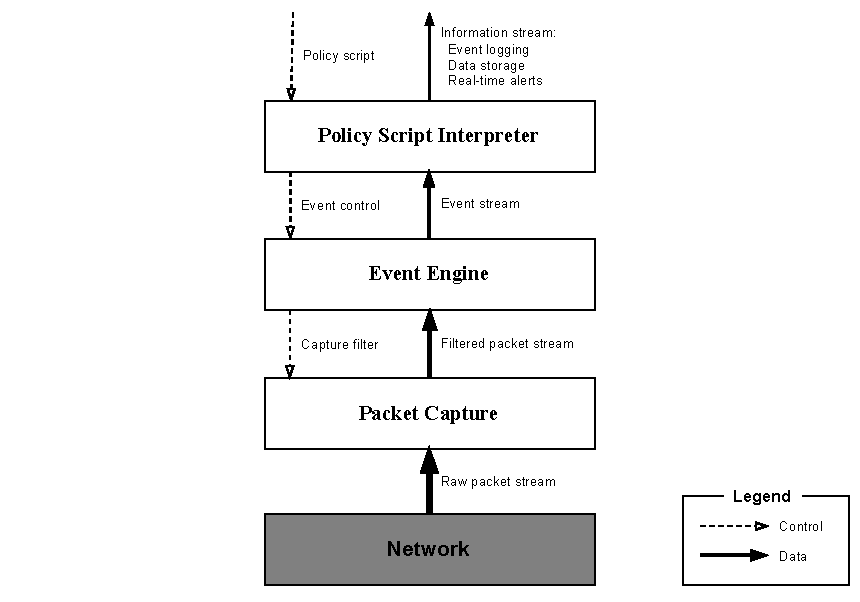
\includegraphics[width=1.0\textwidth]{images/zeek-architecture.pdf}
    \end{center}
    \label{fig:zeek_architecture}
    \legend{Source: \citeonline{Ilha2022}, adapted from \citeonline{Paxson1999}}
\end{figure}

\subsubsection*{Packet Capture}

The \textit{Packet Capture} layer provides an abstraction layer between the network and the \textit{Event Engine}. The original Zeek proposal \cite{Paxson1999} was composed only by the \textit{libpcap} library \cite{Libpcap}. With this extra layer, Zeek is isolated from link-layer technologies, has improved compatibility with other Unix systems, and becomes able to read from packet traces saved as \textit{PCAP} files.

\subsubsection*{Event Engine}
\label{sec:bg:zeek_ee}

The \textit{Event Engine} is the most important layer for our framework (presented in \autoref{cap:rna}) and where our solution is executed. It is responsible for parsing incoming packets and generating events corresponding to those packets. As an example, we cite parsing an incoming ICMP Echo Request and triggering the \texttt{icmp\_echo\_request} event with all the required structured information associated with it.

The internal structure of the \textit{Event Engine}, as explained by \citeonline{Ilha2022}, can be divided into four stages: acquisition, packet analysis, session analysis, and application layer parsing. In the acquisition stage, packets sent by the \textit{Packet Capture} component are received and forwarded to the next stage. In the packet analysis stage, the Packet Analysis Framework (PAF) receives the packets as Protocol Data Units (PDUs) and processes each layer of the packet. In this stage, where lower-layer protocols are analyzed, there is still a clear definition of headers and payloads, and the headers usually contain information of what is the next layer's protocol. Using this information, the PAF processes each header, extracting information and delivering its payload to the next layer until the transport layer is reached. Each analysis layer in the Packet Analysis Framework is called an \textit{Analyzer}. Developers can also create new Analyzers and use them to process new protocols and create different events.

Still in the Event Engine, the session analysis stage creates a \textit{Connection} object that, despite the name, does not only represent a connection as in network terminology but also flows and sessions, for example, ICMP Echo Requests and Replies. This session is then stored and used to associate requests and replies, facilitating parsing for the next stage. After the \textit{session} has been created, the application layer parser selects possible application layer analyzers based on well-known port numbers. Since services are not strictly bound to specific ports, the application layer parser is able to dynamically identify application layer protocols using Dynamic Protocol Detection (DPD), which was introduced by \citeonline{Dreger2006}. Throughout the whole execution of the \textit{Event Engine}, it generates events that have semantic value, and that will be handled by the Policy Script Interpreter (PSI). These events vary from lower-level events, such as a TCP connection established, with the \texttt{connection\_established} event, up to application-layer protocols, for example, an FTP Request and Reply, represented respectively by the \texttt{ftp\_request} and  \texttt{ftp\_reply} events.


\subsubsection*{Policy Script Interpreter}
\label{sec:bg:zeek_psi}

The \textit{Policy Script Interpreter} is an event-driven script interpreter. It processes the events that were triggered by the \textit{Event Engine} using scripts written in a domain-specific language called ZeekScript. To process events, scripts define \textit{event handlers}, similar to functions that process the events to generate logs and alerts. Zeek comes with multiple built-in scripts, such as those for FTP Bruteforce detection, traceroute detection, and others. Users can also write scripts and run their policies.


\subsubsection*{Candidate Operations for Offloading}
\label{sec:bg:zeek_candidate_operations}

In our project, we focus on offloading certain operations of the Zeek system. As \citeonline{Ilha2022} describes in his thesis, the best candidate operations for PDP offloading are those related to the Packet Capture and Event Engine layers. In these layers, the best suitable operations are parsing of protocols up to the transport layer (Ethernet, IPv4, UDP, and others), packet filtering, and lightweight packet inspection \cite{Ilha2022}.

\section{Programmable Data Planes and the P4 Language}
\label{sec:bg:pdp}

% A common misconception about Software Defined Networks (SDN) was about how programmable they were. While not entirely incorrect, this assumption revealed more complex problems as stated by \citeonline{Cordeiro2017}: devices were programmable to a certain point, but developers were limited by a set of protocols and functions that were supported by the target ASICs. Furthermore, OpenFlow API upgrades usually required hardware design changes to the ASICs, slowing down the evolution of this technology.

Programmable Data Planes (PDPs) emerged as a solution to program Software Defined Network (SDN) devices even further, allowing network operators to define protocols and network flow, effectively programming them. Domain-specific languages (DSLs) were developed to program these devices, two notable mentions are POF \cite{Song2013} and P4 \cite{Bosshart2014}. In this project, we focus on P4.


% \subsection{P4 Language}
\label{sec:bg:p4}

P4 stands for \textit{Programming Protocol-Independent Packet Processing}. It was proposed by \citeonline{Bosshart2014} and is a domain-specific language for programming network devices. P4 provides an abstraction for packet parsing and processing by providing a generalized forwarding model \cite{Cordeiro2017}. It is also target-independent and can be executed in different types of switches.

A P4 program is organized into three sections: (a) \textit{data declaration}, (b) \textit{parser logic}, and (c) \textit{match+action tables and control flow} \cite{Cordeiro2017}. These sections can be seen in \autoref{fig:p4_model}. The \textit{data declaration} section defines all required data structures: the headers and the meta-data. These structures are mapped to a header and meta-data bus, which is used throughout the whole pipeline. The definition of a P4 structure is similar to a \textit{struct} definition in C, i.e., a structure can contain multiple data fields, and each field has a type and a length. Differently from C, whose types have sizes expressed in bytes, P4 type sizes are defined by the number of bits. The \textit{parser logic} specifies how packets are parsed and deparsed. This definition uses a state machine to define parsing states, progressing from one protocol to another. Finally, the \textit{match+action tables and control flow} defines the control flow of the ingress and egress pipelines. In this section, it is possible to define routing rules and forward packets to specific ports. This is done using \textit{match+action} tables, which match specific header field values to actions to be executed.

\begin{figure}[H]
    \caption{P4 Forwarding Model}
    \begin{center}
        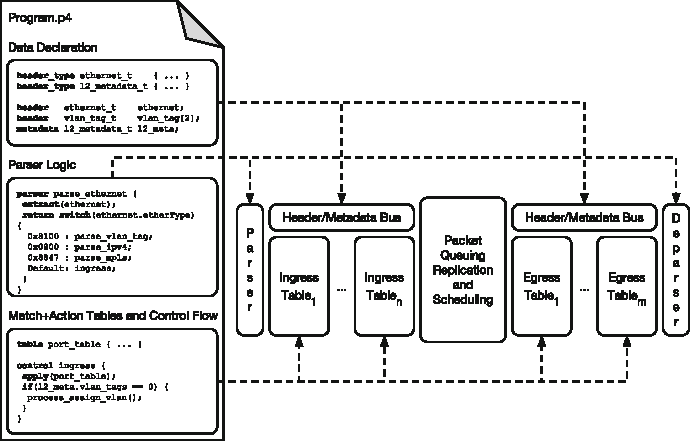
\includegraphics[width=1.0\textwidth]{images/p4model.pdf}
    \end{center}
    \label{fig:p4_model}
    \legend{Source: \citeonline{Cordeiro2017}, adapted from \citeonline{Kim2016}.}
\end{figure}
